\section{Evaluation}
\label{sec:evaluation}

In this section, we present a comprehensive overview of our experimental results. We evaluate the performance of GEM on our two experimental testbeds. We attempt to answer the following questions :

\begin{itemize}

\item What is the number of power-levels that we should use in GEM i.e what is the value of K (mentioned in Section \ref{subsec:latentvariablesfortargetlocationsandpowerlevels} above) that we should use when we run GEM on the back end localization server. 
\item How does the localization accuracy vary as the size of the learning data-set increases.
\item GEM accuracy for heterogenous devices with unmodelled hardware and power-level characteristics
\item How does GEM perform with respect to a model-based scheme that uses the indoor radio path loss propagation model. This presents a true head-to-head comparison because both the techniques do not need pre-deployment effort and can work on the same granularity of discretization of the target space.
\item How does GEM perform with respect to schemes that build RF signal maps like RADAR and Probabilistic. This experiment shows how the WiFi hardware variance problem can impact the accuracy of RF signal map schemes and also show the impact of training granularity for signal map based schemes.
\item We also study how the mobility of a client can actually improve GEM's localization accuracy. 

\end{itemize}

\subsection{Number of powers levels to use in GEM}
\label{subsec:numberofpowerlevelstouseingem}

As mentioned in Section \ref{subsec:datacollectionmethodology} above, the CEWIT testbed has 45 distinct locations and CSD has 27 distinct locations, and for each distinct location on the map and for each device type we have a set of 200 RSS tuples. We divide these 200 tuples into two sets of 100 tuples each: one for learning the GEM parameters and the other for testing the GEM localization results. Each device type is considered separately. Figure \ref{fig:powerlevelsvserrordistance} shows the results of the average error distance (in meters) for the four devices across varying number of power levels used in GEM. We see that the average error distance hits a plateau after K = 31. This is an interesting result because it helps us bound the number of power levels to use. We use a value of K = 45 in the subsequent experiments. 

\subsection{Localization accuracy as a function of the learning set size in GEM}
\label{subsec:localizationaccuracyasafunctionofthelearningsetsizeingem}

\begin{figure}[h!]
\centering
  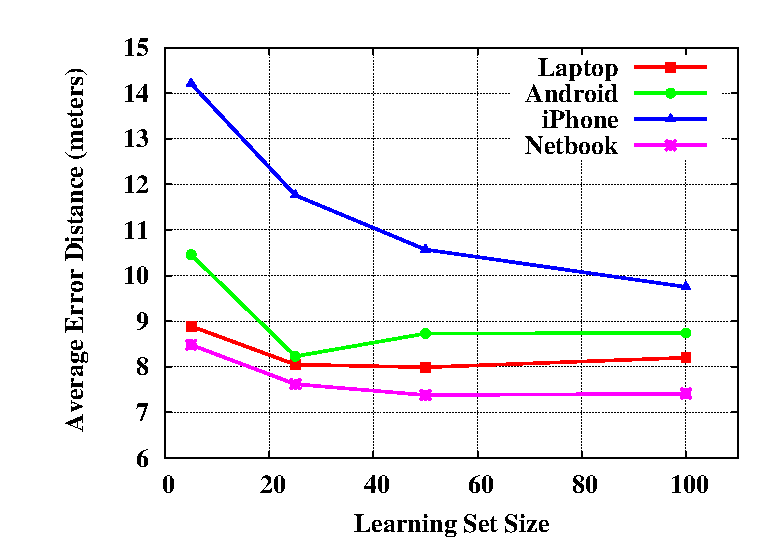
\epsfig{file=Figs4Paper/CEWIT/LearningSize4Paper_CEWIT/LearningSetSize_cewit.eps, height=1.5in, width=2.5in}
  \caption{Average Error distance on the CEWIT Dataset as a function of the learning set size}
  \label{fig:learningsetsizevserrordistance}
\end{figure}

Having fixed the number of power levels to use, we now study how the size of the learning data-set changes the average error distance. Recollect here that as part of our data collection methodology, we have 200 RSS tuples for every location on the map for each of the four device types. This time we again divide the 200 tuples into two sets : one set for learning and the other for testing. The test set size is kept fixed at 100 RSS tuples. From the remaining tuples, the learning set size is varied from 2 tuples going up to 100 tuples. Each device type is considered separately. Figure \ref{fig:learningsetsizevserrordistance} shows the results of the average error distance (in meters) in the CEWIT testbed as the size of the learning set varies. We observe that for all the four devices, the average error does not vary much as the as we move from 50 training samples to 100 training samples. The CSD testbed results (not included here) converged after 25 training samples itself. The experiments which follow have been done keeping the GEM learning set size at 100 and using the remaining 100 samples for testing the localization accuracy.  

\subsection{GEM accuracy for heterogeneous devices}
\label{subsec:gemaccuracyforheterogeneousdevices}

\begin{figure*}
	\centering
	      \subfloat[CEWIT]{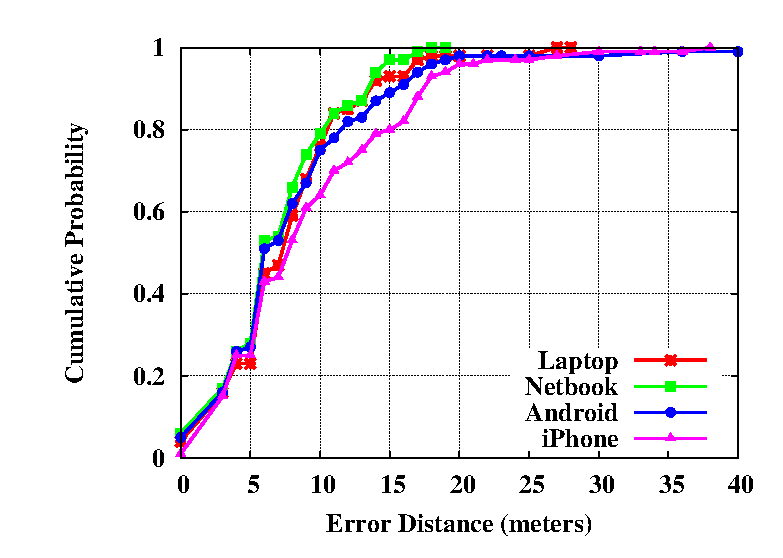
\includegraphics[height=1.5in, width=2.5in]{Figs4Paper/CEWIT/Gem4Devices_CEWIT/4Devices_cewit.eps}}
	      \subfloat[CSD]{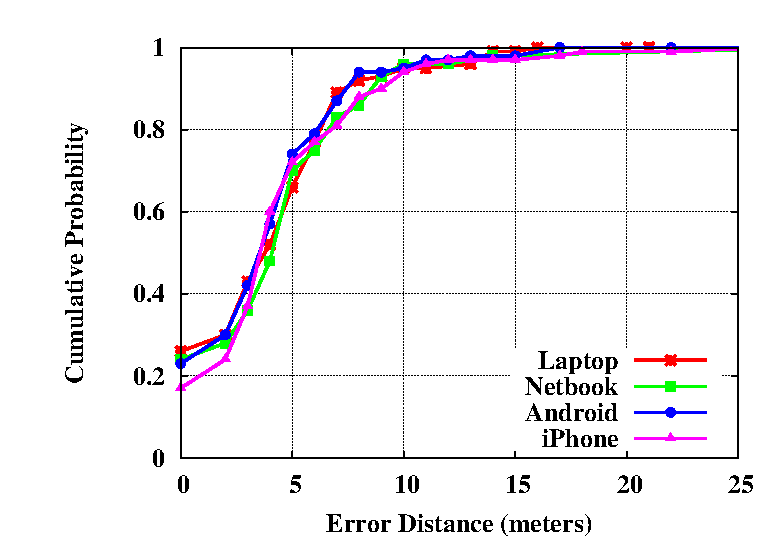
\includegraphics[height=1.5in, width=2.5in]{Figs4Paper/CSD/Gem4Devices_CSD/4Devices_csd.eps}}
	\caption{GEM location accuracy for multiple devices}
	\label{fig:gemheterogeneousdevices}
\end{figure*}

Figure \ref{fig:gemheterogeneousdevices} shows how GEM performed across the four test devices \ref{subsubsec:testdevices} on both the testbeds. We see that for both the testbeds, the accuracy estimates are pretty similar for all the devices. Thus we see that GEM can adapt itself for heterogeneous devices working at different power levels. Section \ref{subsec:comparisonswithschemesthatuserfsignalmaps} below shows how RF-signal map based techniques show substantial degradation in accuracy because of hardware variance. 

\subsection{Baseline Comparison with a model-based scheme}
\label{subsec:baselinecomparisonwithamodelbasedscheme}

\begin{figure*}
	\centering
	      \subfloat[CEWIT]{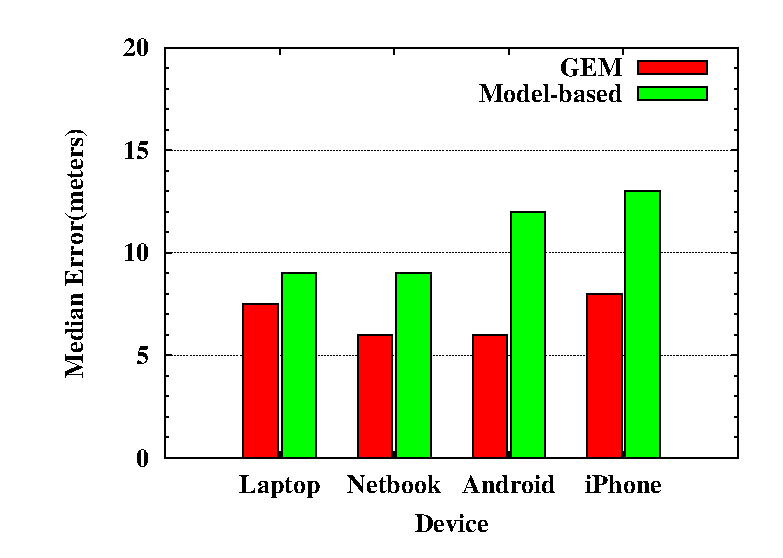
\includegraphics[height=1.5in, width=2.5in]{Figs4Paper/CEWIT/Baseline4Paper_CEWIT/BaselineComparisonsMedianError_cewit.eps}}
	      \subfloat[CSD]{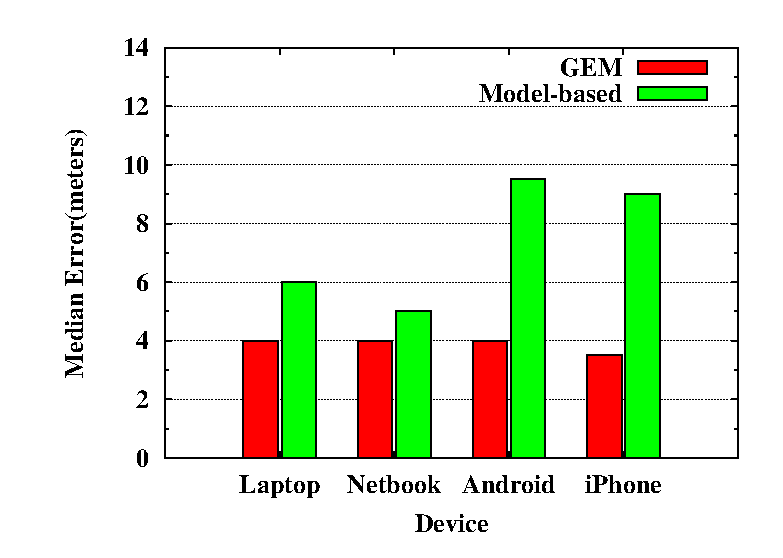
\includegraphics[height=1.5in, width=2.5in]
	      {Figs4Paper/CSD/Baseline4Paper_CSD/BaselineComparisonsMedianError_csd.eps}}
	\caption{Baseline Comparisons}
	\label{fig:baselinecomparisons}
\end{figure*}

% \begin{figure*}
% \begin{minipage}{0.5\textwidth}
% 	{\centering
% 	  \subfloat[Probabilistic]{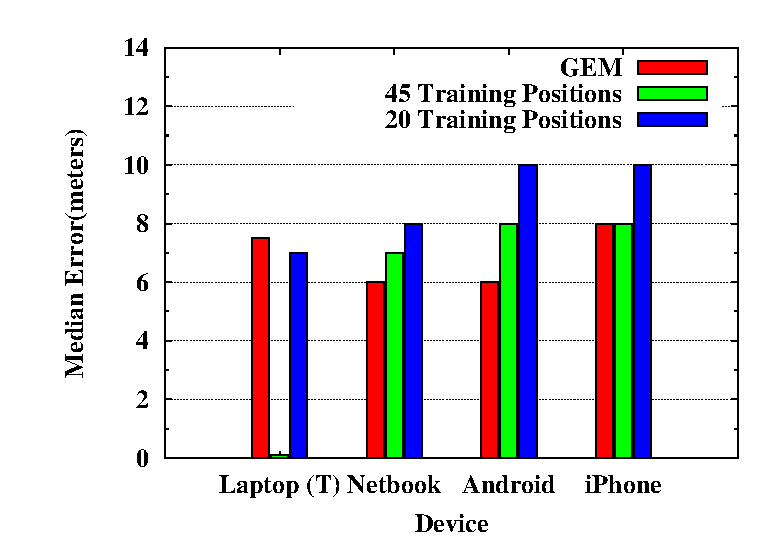
\includegraphics[width=0.5\textwidth]{Figs4Paper/CEWIT/HRComparisons4Paper_CEWIT/HRComparisonsMedianError_Probabilistic_cewit.eps}}
% 	  \subfloat[RADAR]{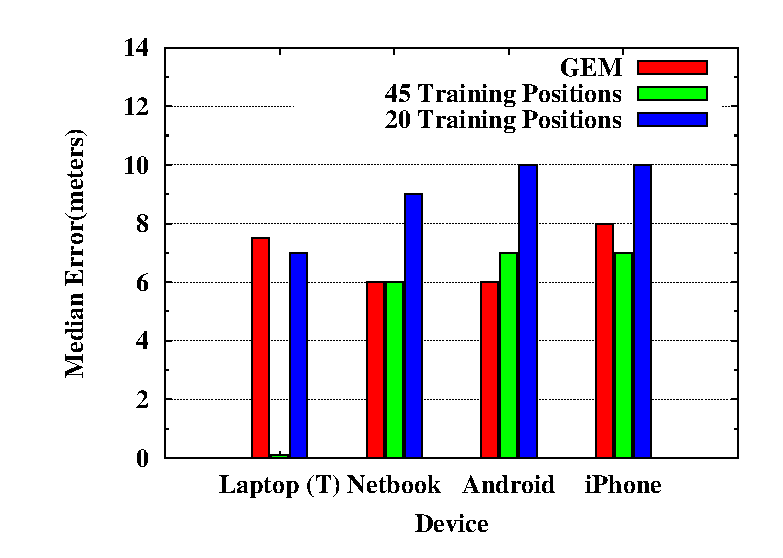
\includegraphics[width=0.5\textwidth]{Figs4Paper/CEWIT/HRComparisons4Paper_CEWIT/HRComparisonsMedianError_RADAR_cewit.eps}}
% 	\caption{Comparisons on the CEWIT Testbed}
% 	\label{fig:HR_on_cewittestbed}
% 	}
% \end{minipage}\quad
% \begin{minipage}{0.5\textwidth}
% 	{\centering
% 		\subfloat[Probabilistic]{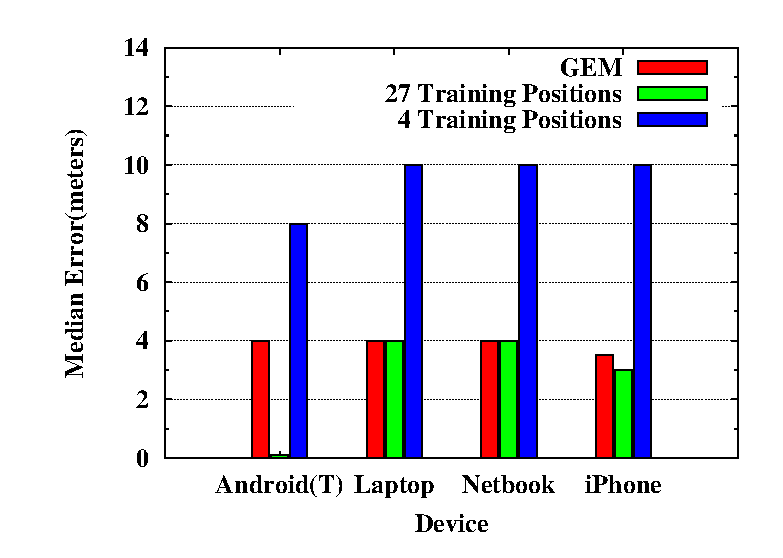
\includegraphics[width=0.5\textwidth]{Figs4Paper/CSD/HRComparisons4Paper_CSD/HRComparisonsMedianError_Probabilistic_csd.eps}}
% 		\subfloat[RADAR]{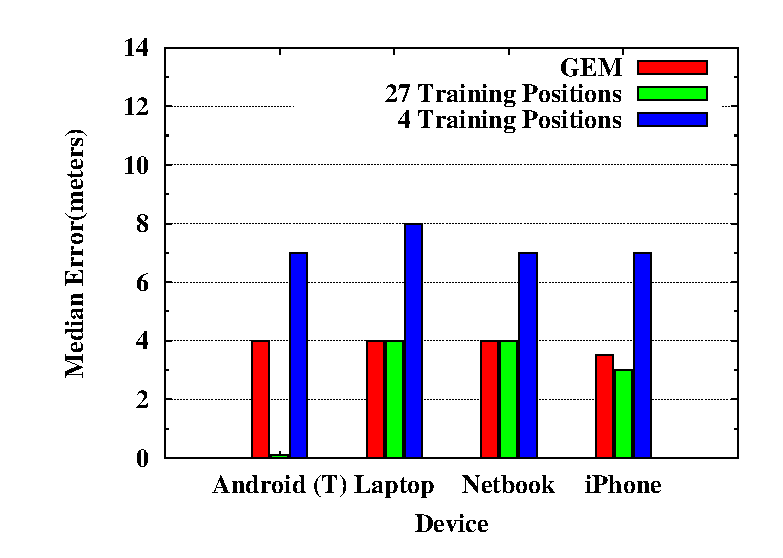
\includegraphics[width=0.5\textwidth]{Figs4Paper/CSD/HRComparisons4Paper_CSD/HRComparisonsMedianError_RADAR_csd.eps}}
% 	\caption{Comparisons on the CSD Testbed}
% 	\label{fig:HR_on_csdtestbed}
% 	}
% \end{minipage}
% \end{figure*}

Here we analyze the performance of GEM with respect to a model-based scheme that uses the indoor radio path loss propagation model (Section \ref{subsec:handlingidentifiabilityinourmodel}). This presents a true head-to-head comparison, because both the techniques do not need pre-deployment effort and can  give a location estimate at the same granularity of discretization of the target space. Both our testbeds, CEWIT and CSD, have been discretized as shown in Figure \ref{fig:experimenttestbed}. There are 267 grid vertices inside the CEWIT testbed roughly every 2.75 meters. The CSD testbed has 36 grid vertices roughly every 3.1 meters. GEM can localize a given target RSS vector to any of these grid vertices. As mentioned in Section \ref{subsec:datacollectionmethodology}, the data for our experimental evaluation is coming from 45 distinct locations on the CEWIT testbed and 27 distinct locations in the CSD testbed. There are 200 RSS tuples for every location on the map for each of the four device types. As mentioned above in Section aa, GEM is using a learning set size of 100 RSS samples with 45 power levels to build the model. Thus the test-set for both the algorithms is remaining 100 RSS tuples from each location. Each device type is evaluated separately.

The log-distance path loss (LDPL) mentioned in Section \ref{subsec:handlingidentifiabilityinourmodel} is used to estimate the RSS that should be observed at a sniffer for each grid vertex inside the target-space. These RSS values are used to initialize GEM, as mentioned in section \ref{subsec:handlingidentifiabilityinourmodel}. The Model-based algorithm also uses these same RSS values with a suitable metric to give a final location estimate. Similar to \cite{Bahl00radar:an}, the model-based algorithm that we use here uses nearest neighbor in signal space (NNSS) as the metric of choice. 

Figure \ref{fig:baselinecomparisons} shows the median error for both techniques. We see that GEM performs better than the model-based scheme across all device types in both the testbeds.

\subsection{Comparisons with schemes that use RF signal maps}
\label{subsec:comparisonswithschemesthatuserfsignalmaps}

\begin{figure*}
	\centering
	      \subfloat[Probabilistic]{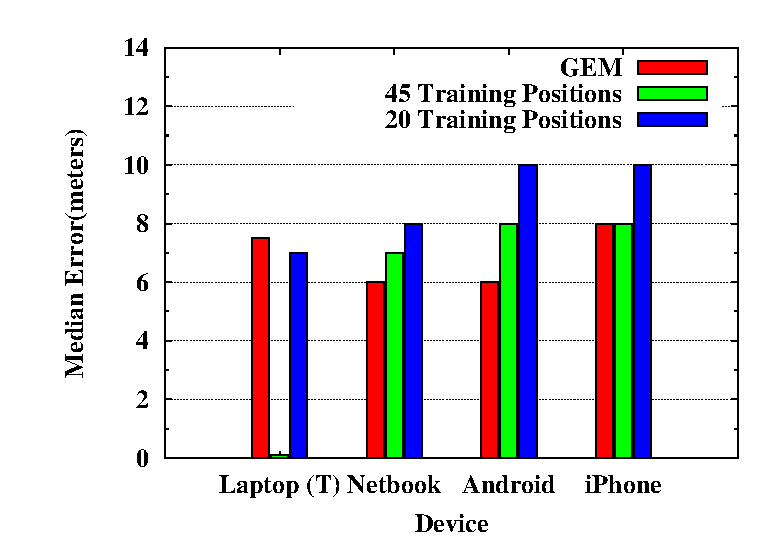
\includegraphics[height=1.5in, width=2.5in]{Figs4Paper/CEWIT/HRComparisons4Paper_CEWIT/HRComparisonsMedianError_Probabilistic_cewit.eps}}
	      \subfloat[RADAR]{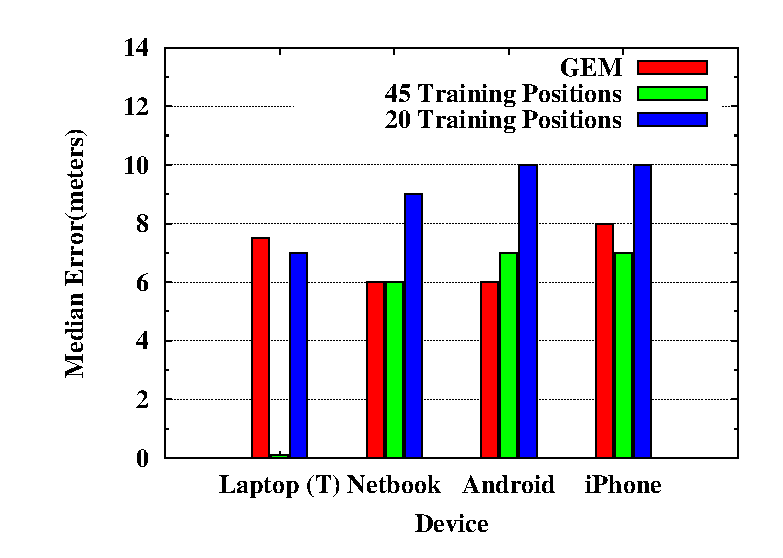
\includegraphics[height=1.5in, width=2.5in]
	      {Figs4Paper/CEWIT/HRComparisons4Paper_CEWIT/HRComparisonsMedianError_RADAR_cewit.eps}}
	\caption{Comparisons on the CEWIT testbed}
	\label{fig:HR_on_cewittestbed}
\end{figure*}

\begin{figure*}
	\centering
	      \subfloat[Probabilistic]{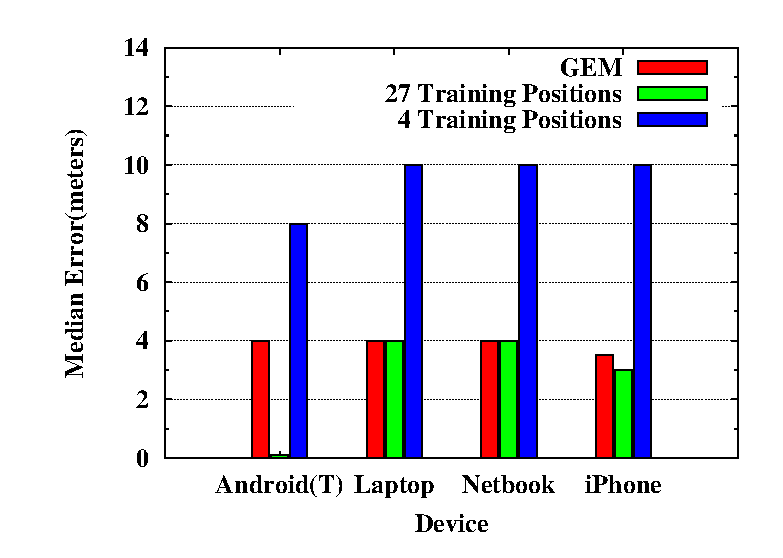
\includegraphics[height=1.5in, width=2.5in]{Figs4Paper/CSD/HRComparisons4Paper_CSD/HRComparisonsMedianError_Probabilistic_csd.eps}}
	      \subfloat[RADAR]{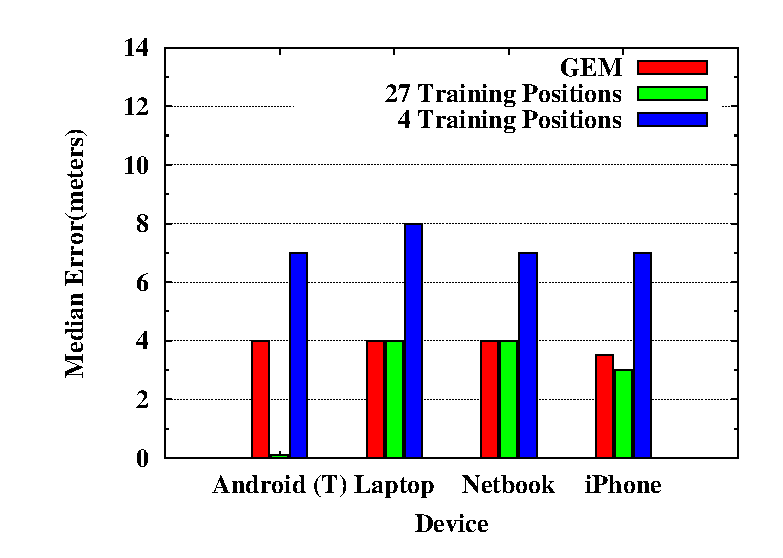
\includegraphics[height=1.5in, width=2.5in]
	      {Figs4Paper/CSD/HRComparisons4Paper_CSD/HRComparisonsMedianError_RADAR_csd.eps}}
	\caption{Comparisons on the CSD testbed}
	\label{fig:HR_on_csdtestbed}
\end{figure*}

We now compare the performance of GEM again two schemes that spend considerable pre-deployment effort in first building an RF signal map from RSS signatures collected from various locations inside the target space. Both schemes differ in the way they handle an incoming signature to provide a location estimate.

\begin{itemize}
\item Deterministic schemes like RADAR \cite{Bahl00radar:an} use the nearest neighbor in signal space (or an average of k-nearest neighbors) as the metric to give a location estimate. 
\item Probabilistic schemes \cite{Haeberlen:2004:PRL:1023720.1023728, Youssef:2008:HLD:1399551.1399558, Roos} on the other hand maintain a probability distribution of the RSS value from various locations. For the incoming signature, a probability distribution is built over the location space and a maximum likelihood estimate is used to determine position. As in \cite{Haeberlen:2004:PRL:1023720.1023728}, we model signal intensity as a normal distribution determined by the location and sniffer pair. 
\end{itemize}

\subsubsection{Discussion}
\label{subsubsec:rfsignalmapdiscussion}

\begin{enumerate}

\item 
For all three techniques that we compare here viz GEM, RADAR and Probabilistic, we consider the best location as our location estimate. We do not consider the weighted average of the top few locations for any of the three techniques compared here. 

\item
To show the WiFi hardware variance problem mentioned in Section \ref{sec:introduction}, we use different devices for location estimation. For the CEWIT testbed, a DELL Laptop was used to train the radio map during the {\it `offline' phase}. In the CSD testbed, an android phone was used to build the radio map. Based on the radio maps, four different device types are used to give location estimates. 

\item
As mentioned in Section \ref{subsec:datacollectionmethodology}, the data for our experimental evaluation is coming from 45 distinct locations on the CEWIT testbed and 27 distinct locations in the CSD testbed. 

For RADAR and Probabilistic, we try to understand the effect of the granularity of training locations on the final location estimate. We consider two scenarios : one optimistic and the other more realistic. In the first scenario, we consider the optimistic secnario where the training and test data sets (mentioned below) are collected at the same physical locations, e.g on the CEWIT testbed, the signal map is built from the same 45 distinct locations where the position estimation is being done. The second scenario, is the more realistic scenario where the training is done from only a subset of the test locations. Thus the testing locations are no longer strictly co-located with the training locations. In the CEWIT testbed, the training is done from 20 locations (out of the 45 possible) roughly every 10.3 meters apart. In the CSD testbed, the subset comprises of 4 locations (out of the 27 possible) roughly every 12.7 meters apart.  We note here that GEM on the other hand requires no training effort. For GEM we use the same discretization of the target space that we use in section \ref{subsec:baselinecomparisonwithamodelbasedscheme} i.e the GEM location estimate can be on any of the grid points inside the building.

\item
There are 200 RSS tuples for every location on the map for each of the four device types. We divide these 200 tuples into two disjoint sets of 100 tuples each. The first set is used by RADAR and Probabilistic to build their RF signal maps while GEM uses it as the learning data to build the localization model.  The second set of 100 tuples from each location is used as the test data for all three algorithms. Every device type is evaluated separately. 

\end{enumerate}

\begin{figure*}
	\centering
		\subfloat[CEWIT]{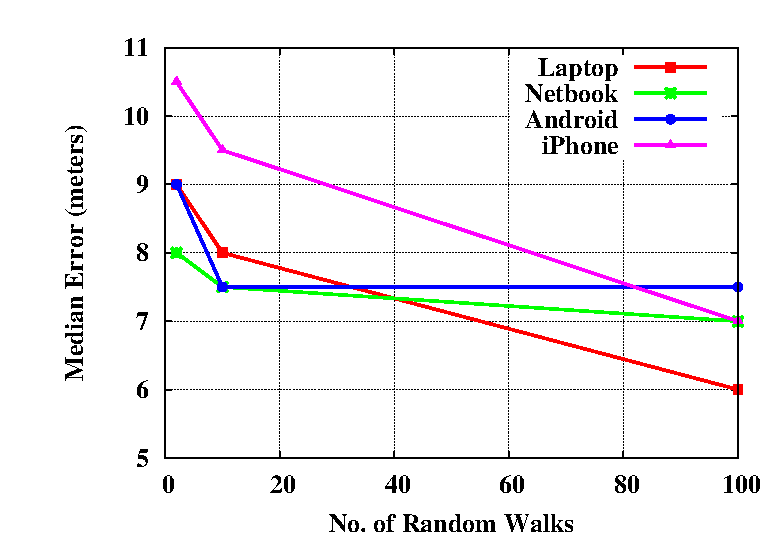
\includegraphics[height=1.5in, width=2.5in]{Figs4Paper/CEWIT/MobilityPlot4paper_CEWIT/Mobility_cewit.eps}}
		\subfloat[CSD]{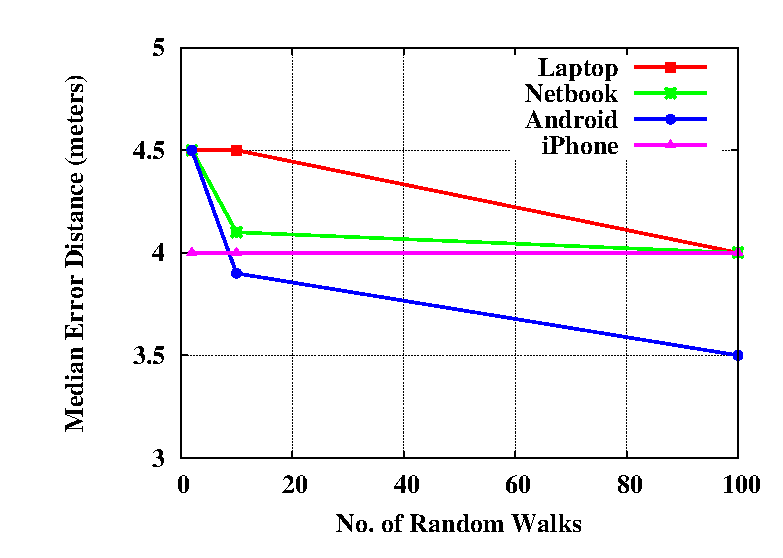
\includegraphics[height=1.5in, width=2.5in]{Figs4Paper/CSD/MobilityPlot4paper_CSD/Mobility_csd.eps}}
	\caption{Mobility}
	\label{fig:mobility}
\end{figure*}

\subsubsection{Observations}
\label{subsubsec:rfsignalmapobservations}

Figure \ref{fig:HR_on_cewittestbed} and Figure \ref{fig:HR_on_csdtestbed} shows the median error comparison between the three techniques . We make some interesting observations here:
 
\begin{itemize}

\item Hardware variance is a major issue for both RADAR and Probabilistic. When the same device is used for training and testing, the median error is zero. For other devices it jumps up dramatically. This is a critical problem for such techniques because a real-world deployment would be typically unaware of the device type being localized. In fact, we see GEM performing as good as RADAR and Probabilistic for other device types. This is particularly promising because unlike RADAR and Probabilistic, GEM did not have the overhead of a pre-deployment effort.

\item When the granularity of sampling is reduced, RADAR and Probabilistic start showing substantially poorer accuracy estimates. Thus location estimates for such techniques are tightly bound to the granularity of the training effort. This makes them unattractive for performing localization in large target spaces. A heavy pre-deployment effort also make these techniques difficult to maintain and  update in a dynamic environment.

\end{itemize}

\subsection{Impact of Mobility on GEM's localization accuracy}
\label{subsec:impactofmobilityongemslocalizationaccuracy}

In this experiment we try to understand how the mobility of a client can effect the location estimates made by GEM. To create the test data set, a user initially walks across all distinct location on the map, making 100 ping transmissions from each location. This forms our test data set which is basically a union of 100 RSS tuples from each distinct location on the map.  Now we try to observe the effect of client mobility in localizing this test data set. To do this, the user follows a random walk scheme. In each random walk, the user visits every distinct location in the building floor once, and makes a single ping transmission from that location. This serves as the learning data-set for GEM, in order to build a model for the device and give location estimates for the test set. 

We evaluate this scheme on both testbeds across four different devices. Figure \ref{fig:mobility} shows how the median error of the test data set varies as the mobility (i.e the number of random walks) increases. We observe that mobility actually helps GEM localization accuracy.

